\documentclass{beamer}

\usetheme{Madrid}
\usecolortheme{default}
\setbeamercovered{transparent}

\title{The Evolution of Computing Paradigms}
\subtitle{A Comprehensive History of Programming Languages}
\author{Wojciech Fiołka, Paweł Kojma, Michał Bednarz, Jakub
Chomiczewski, Filip Rabiega}
\institute{Department of Computer Science}
\date{\today}

\begin{document}

\frame{\titlepage}

\begin{frame}{Foundations of programming}
  \begin{columns}
    \column{0.55\textwidth}
    Programming began as the bridge between mathematical theory and
    physical hardware. We moved from 19th-century algorithms to the
    reality of binary machine code, eventually developing assemblers
    to translate human mnemonics into logic. This era established the
    core necessity of abstraction to manage growing complexity.

    \column{0.4\textwidth}
    \centering
    \includegraphics[width=\textwidth]{img/foundations_of_programming.jpg}
    \par\vspace{0.2cm}
    \footnotesize{Ancient programmer}
  \end{columns}
\end{frame}

\begin{frame}{First languages}
  \begin{columns}
    \column{0.55\textwidth}
    The "Software Crisis" forced a leap toward high-level
    portability. This period defined the three pillars of computing:
    high-speed calculation, business data processing, and the birth
    of functional programming. By introducing symbolic logic and
    automated memory management, these languages broke the rigid link
    between code and machine architecture.

    \column{0.4\textwidth}
    \centering
    \includegraphics[width=\textwidth]{img/first_languages.png}
    \par\vspace{0.2cm}
    \footnotesize{Software Crisis}
  \end{columns}
\end{frame}

\begin{frame}{LISP}
  \begin{columns}
    \column{0.4\textwidth}
    \centering
    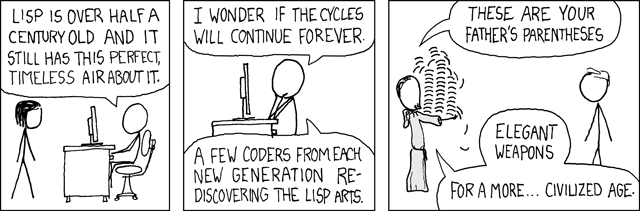
\includegraphics[width=\textwidth]{img/lisp.png}
    \par\vspace{0.2cm}
    \footnotesize{The average LISP experience}

    \column{0.55\textwidth}
    First functional language, introduced garbage
    collection and heap allocation, symbolic computing used for
    reasearching AI in the US, free from Von Neumannean notions of variables,
    assignments, gotos etc. It didn't catch on in the 50s and 60s due
    to hardware limitations and lack of tooling at the time, it has however
    spawned many dialects over the years.
  \end{columns}
\end{frame}

\begin{frame}{Structure and logic}
  \begin{columns}
    \column{0.4\textwidth}
    \centering
    \includegraphics[width=\textwidth]{img/structure_and_logic.png}
    \par\vspace{0.2cm}
    \footnotesize{Spaghetti code}

    \column{0.55\textwidth}
    To combat unmanageable "spaghetti code," the industry embraced
    modularity and formal flow control. This era replaced arbitrary
    jumps with nested logic and structured blocks. It proved that
    programming could be a disciplined engineering craft, focused on
    readable, verifiable execution paths.

  \end{columns}
\end{frame}

\begin{frame}{Haskell}
  \begin{columns}
    \column{0.55\textwidth}
    It was designed to unify the functional programming community, offering a
    purely functional approach while advancing sophisticated type systems. It
    also introduced lazy evaluation, a feature that was quite unusual at the
    time.

    \column{0.4\textwidth}
    \centering
    
\includegraphics[width=\textwidth]{img/haskell.jpg}
    \par\vspace{0.2cm}
    \footnotesize{The joys of purely functional programming}
  \end{columns}
\end{frame}

\begin{frame}{Object oriented shift}
  \begin{columns}
    \column{0.55\textwidth}
    Complexity management shifted from procedural steps to
    data-centric encapsulation. By bundling state and behavior into
    objects, developers gained a new way to build and maintain
    massive systems. This paradigm shift redefined how software is
    architected, focusing on modeling real-world entities.

    \column{0.4\textwidth}
    \centering
    \includegraphics[width=\textwidth]{img/object_oriented_shift.png}
    \par\vspace{0.1cm}
    \footnotesize{Object oriented design patterns}
  \end{columns}
\end{frame}

\begin{frame}{OCaml}
  \begin{columns}
    \column{0.4\textwidth}
    \centering
    
\includegraphics[width=\textwidth]{img/ocaml.jpg}
    \par\vspace{0.2cm}
    \footnotesize{funni comment}

    \column{0.55\textwidth}
    It was designed to extend the ML family by combining functional
    programming with practical features for real-world use. It offers a strong
    static type system with powerful type inference, while also supporting an
    object-oriented style, making it both functional and object-oriented. This
    balance allows it to be expressive and efficient, suitable for both research
    and industrial applications.
  \end{columns}
\end{frame}

\begin{frame}{Scripting and productivity boom}
  \begin{columns}
    \column{0.55\textwidth}
    As the internet scaled, the focus shifted from machine efficiency
    to "developer velocity." High-level scripting and virtual
    machines prioritized human time, allowing for rapid prototyping
    and platform independence. Programming became more about the
    speed of turning ideas into functional software than managing
    hardware constraints.

    \column{0.4\textwidth}
    \centering
    \includegraphics[width=\textwidth]{img/scripting_and_productivity.png}
    \par\vspace{0.2cm}
    \footnotesize{Node.js programming environment}
  \end{columns}
\end{frame}

\begin{frame}{Contemporary language trends}
  \begin{columns}
    \column{0.4\textwidth}
    \centering
    \includegraphics[width=\textwidth]{img/rust_pipeline.png}
    \par\vspace{0.2cm}
    \footnotesize{Path of a Rust programmer}

    \column{0.55\textwidth}
    Modern development focuses on "guardrails" eliminating memory
    errors and concurrency bugs at the compiler level. This is also
    an era of refined research; projects like Fram (UWr) are pushing
    the ML tradition forward by using algebraic effects and implicit
    parameters to handle side effects with modular, ergonomic precision.
  \end{columns}
\end{frame}

\begin{frame}{Future of programming}
  \begin{columns}
    \column{0.4\textwidth}
    \centering
    \includegraphics[width=\textwidth]{img/future_of_programming.png}
    \par\vspace{0.2cm}
    \footnotesize{Future of programming with LLMs}

    \column{0.55\textwidth}
    We are moving from "writing" code to "orchestrating" intent. The
    rise of AI agents shifts the programmer’s role toward high-level
    architecture, while the dawn of quantum computing demands an
    entirely new logical framework, shifting our focus from bits and
    states to the complex probabilities of qubits and superposition.
  \end{columns}
\end{frame}

\end{document}
